\documentclass{article}
\usepackage[parfill]{parskip}
\usepackage{url}
\usepackage{courier}
\usepackage{glossaries}
\usepackage{mathtools}
\usepackage{xcolor}
\usepackage{tcolorbox}
\usepackage{tikz}
\usetikzlibrary{positioning}

\begin{document}
\section{Abstract}

\tableofcontents
\section{Introduction}
Over the past 50 years, UNIX and its descendent Operating Systems have created a set of standardised patterns for how computers interact with themselves, each other, and the outside world.
These patterns; files, threads, device drivers, etc. are so powerful that computing devices are classified first by whether or not they are capable of supporting them.
Microprocessors typically support multitasking, networking, and are connected to large amounts of volatile and non-volatile storage.
Microcontrollers, on the other hand, tend to be realtime, with primitive networking and EEPROM storage that often cannot be rewritten at runtime.

As moore's law slows and the graph of computing power over time begins to flatten, semiconductor manufacturers have created new devices.
Because waiting for cheaper hardware is no longer a valid \lq optimization' stratergy, manufacturers have begun adding microprocessor-like capabilities to microcontrollers.
Although these new devices are traditionally classified as microcontrollers, theese new capabilities blur the line between the microcontrollers and microprocessors.
The \lq super-mircocontroller' used in this project was the Espressif systems ESP-32.

The goal of this project is to create the first of a new set of patterns designed from the ground up for the new hardware; to encapsulate storage, code execution, IO and communication in a simple to use and extensible platform.
Because implementing an entire platform of this scale is outside of the scope of a single-module dissertation, this project is more a proof-of-concept than a final version.
Concessions have been made to simplicity to allow for experimentation, meaning that no guarantees can be made about security or speed.
The project aims, however, to be well tested and stable.

\pagebreak
\section{Literature Review}


\section{Methodology}
\subsection{Problem Description}
\subsection{Technologies used}
\subsubsection{ESP-32}

Released in 2016, the Espressif Systems ESP-32 is a powerful dual-core microcontroller.
It is based a Cadence IP core, which is in turn based on the Xtensa instruction set \cite{32datasheet}.
This instruction set is often used for specalist Digital Signal Processing hardware because it supports SIMD and customised instructions \cite{lx6datasheet}.
Although it is RISC, it generally complies programs into fewer instructions than arm because it allows for more flexible memory manipulation.
A comparison between the ESP-32, Arduino Uno (with an ATmega328P mircocontroller), and Pixel 3A (with a Snapdragon 670 microprocessor) follows;

\begin{table}[h]
\begin{tabular}{l|lll}
						& Arduino Uno		& ESP-32		& Pixel 3a		\\ \hline
Clock Frequency			& 16 MHz			& 240 MHz		& 1700 MHz		\\ \hline
RAM						& 32 KB				& 520 KB		& 4 GB			\\ \hline
WiFi 					& N 				& \textbf{Y}	& \textbf{Y}	\\ \hline
Hardware multithreading	& N 				& \textbf{Y}	& \textbf{Y}	\\ \hline
Bluetooth				& N 				& \textbf{Y}	& \textbf{Y}	\\ \hline
Rewritable storage		& N 				& \textbf{Y}	& \textbf{Y}	\\ \hline
External SD Card		& N 				& \textbf{Y}	& N				\\ \hline
Ethernet				& N 				& \textbf{Y}	& N				\\ \hline
IO pins					& \textbf{20/22}	& \textbf{39}	& N/A			\\

\end{tabular}
\end{table}

\emph{Note: Missing functionality can be added using external electronics}

In addition to the I/O in the above table, the ESP-32 also supports SPI, I\textsuperscript{2}S, I\textsuperscript{2}C, CAN, as well as dedicated hardware for accelerating hashing, encryption, signing, decryption, and cryptographic random number generation.
The entropy source for the RNG is background noise collected from the RF module.

The ESP-IDF (IoT Development Framework) is a library provided by Espressif systems. It integrates into and extends the dedicated hardware provided by the processor.
For example, Writing code against the WiFi transceiver requires using the IDF's TCP, UDP, or HTTP library.
Similarly, cryptography support is provided through the IDF's port of mbedtls, and the SPI flash is exposed through several libraries inside of the IDF.

\subsubsection{SPIFFS}

One particularly useful part of the IDF is SPIFFS (SPI Flash FileSystem).
It exposes a section of the SPI non-volatile flash storage as a basic filesystem.
SPIFFS does not support directories, so a file saved as \texttt{/spiffs/a/b/c.txt} would be in the same directory as \texttt{/spiffs/d.txt}.
SPIFFS also does not support journaling, so if power is removed halfway through a write operation, it must be reformatted.
This means that the ability to restore from a complete format is important.
SPIFFS also limits filenames to 31 characters.

The Nihilo platform hides file I/O behind trees of values, objects and arrays, using JSON files.
The cJson package is included in IDF, and was used for all storage in this project.

\subsubsection{WebAssembly/wasm3}

Although the target of this project is the ESP-32, the goal is for it to be architecture agnostic.
This includes both running on different instruction sets and running on different types of computer including desktops and servers.
The problem of targeting different types of device using the same standard is similar to the problem websites were made to solve.
The environment of the web adds the bonus that browser-based runtimes are sandboxed and have been aggressivley tested for vulnerabilities.
The traditionally accepted web language, used in both NodeJS and IoT-DSA, is Javascript.

Javascript, though popular, is a bad fit for creating this platform.
Efficent runtimes are large and are usually themselves very architecture-dependent.
In addition, embedded developers tend to favour strong, static typing and DIY memory management, historically meaning C but a variety of newer languages such as Rust, Golang, and C++ have also been gaining popularity.
Emscripten and later WebAssembly were created to enable C-style languages on the web.
The former compiles code to a highly optimizable subset of Javascript, asm.js, which is backwards compatible with any Javascript engine but runs at near-native speeds in a supported one \cite{asm}.
The latter is an extension to asm.js which abandons the link to Javascript entirely, compiling code to a new instruction set running on an idealised processor \cite{wasm}.

WebAssembly (often shortened to wasm) is intended to be executed using a AOT (ahead of time)  or JIT (just in time) compiler, translating the abstract wasm instructions into real instructions to be executed on the processor.
The difference between JIT and AOT is that AOTs translate into code before the program is run, while JITs compile just before the code is executed.
JITs are generally faster because they can optimize based not just on static analysis but also the actual, runtime values of the variables being used.
Slower than both types of compiler are interpreters, which iterate over the commands one by one and execute them by calling functions associated with each command.
Although compilers are prefereable, they are harder to implment, harder to secure, harder to debug, and require porting to each instruction set they must run on.
Because of wasm's relative immaturity, only two partially implemented runtimes exist for embedded architectures;
\begin{itemize}
\item WebAssembly Micro Runtime (WAMR), the official Bytecode Alliance runtime for running webassembly on microcontrollers.
WAMR can run both in AOT and interpreter mode.
It WAMR is well implemented, but lacks ESP-IDF support and porting the entire runtime is beyond the scope of this project.
\item Wasm3, an unofficial interpreter for WebAssembly. 
Although wasm3 is less professionally implemented, it has excellent support for ESP-IDF.
Its simplicity also aids in modifications and experiments. 
\end{itemize}

Wasm3 was chosen for this project.

\subsection{Implementation}
\subsubsection{Machines}

The fundamental, indivisible unit of Nihilo is the machine; many machines can be stored on each physical device. Machines are an idealised and abstract version of a computer; communication, execution, and data storage all happen at the machine level. Communication between and within devices happens from one machine to another, using remote procedure calls. Within SPIFFS, each machine is represented by a JSON and WASM file; the JSON storing data and the WASM storing code.

Many machines can be stored on one device, potentially including machines providing self-contained units of functionality developed by third parties. In order to be useful, however, the user must create a single, master machine, tying together all of the others. When the device boots it will connect to WiFi, load the master machine, and execute its \texttt{entry()} function. This can then be used to instantiate functionality in other machines.

\subsubsection{Security Model}

For security purposes, machines are sandboxed from eachother, but have absolute power over their internal environment. This is because machines are from a single origin, analogous to how javascript has absolute power over its own HTML under the same origin policy, but can only communicate with others through specific channels. Every machine in Nihilo has an asymmetric keypair. Because every communication in Nihilo has an origin and destination machine, it can be cryptographically verified that;
\begin{itemize}
\item The message was sent only by the stated origin.
\item The message can be read only by the stated destination.
\end{itemize}

RSA (Rivest–Shamir–Adleman)\cite{rsa}, the industry standard algorithm for asymmetric cryptography, was initially considered for this task. Although RSA is very secure, developing for the microcontroller platform exposes a set of issues with RSA which are usually hidden by the power of modern computers. The first of these problems is that key generation (keygen) is profoundly computationally intensive. RSA's hardness assumption is a stronger version of its keygen process; both involving the factorisation of very large numbers. RSA keygen on the ESP-32 takes in excess of 20 seconds.

ECC \cite{ecc}(Elliptic Curve Cryptography) is a set of cryptographic primitives based on modular elliptic curves. ECC was built into an asymmetric cryptosystem called ECDH (Elliptic Curve Diffie-Hellman), which is far more computationally efficent than RSA. It has a number of advantages over RSA;
\begin{itemize}
\item Keygen is finished in 200ms, a 100 times speedup.
\item ECDH is not an encryption algorithm, but a key agreement protocol where all of the necassary information is already embedded in the public key of the peer. Both RSA and ECDH need a symmetric encryption algorithm for the bulk exchange of data, but RSA requires a dedicated protocol to send the encrypted symmetric key from one peer to the other while ECDH does not.
\item ECC curve25519 public and private keys are 32 bytes long, as opposed to at least 128 bytes with RSA.
\item Every pair of peers has its own secret, which requires the private key of one and the public key of the other. This negates the need for a dedicated signature, which would be required under RSA.
\end{itemize}

The sum of these advantages is a massively streamlined communication process compared to one implemented using RSA. The 200ms keygen means that machines can be created much faster, while the implicit signature and key exchange negate the need of an SSL-style intermediate layer.

Because the cryptographic verification requires holding the keypair, ownership of the keypair is for all intents and purposes ownership of the machine. The security model breaks down if multiple devices hold the same keypair, so transferring private keys between devices or exposing them to WASM code is \textbf{explicitly forbidden}.

There are two desired capabilities of any asymmetric encryption scheme; security and authentication. Security is the knowledge that only the recipient of the message can decode it. Authentication is the knowledge that the recipient is who they say they are. The ECDH algorithm used by the Nihilo runtime implicitly provides security, but not authentication, which would require one of;

\begin{itemize}
\item A dedicated Public Key Infrastructure (PKI), built on ECC, allowing any claims of identity to be traced back to a common trusted third party.
\item An integration into an existing PKI, such as SSL.
\item A hybrid approach, where trust is rooted in SSL but becomes transferred to Nihilo at some point down the chain to the device attempting to authenticate.
\end{itemize}

Ultimatley, the alternative to building a PKI chosen was using the public keys as the primary identifier of a machine. Because there is no known mechanism to efficently forge a public key, the resulting keys are almost guaranteed to be unique.

Once ECDH has been run, transforming a keypair of one machine and a public key of the other into a shared secret, the message must be symmetrically encrypted. The algorithm chosen was AES\cite{aes}, an efficent block cipher. AES works one block at a time, applying encryption to 16 bytes, then moving on to the next 16 bytes. The original implementation of AES, called ECB mode, had a flaw where identical blocks were encrypted as identical ciphertext, exposing ECB encryption to a variety of attacks, which were rectified with CBC mode. This mode uses the previous block to help encrypt the next, so requires an initialization vector to randomise the first block.

Because the initialization vector is required to decrypt the data, it is included in Nihilo as the 0th block of any encrypted data. If \(x\) is the length of the unencrypted data and b is the block size (16 bytes), the formula for calculating the length of encrypted data is as follows;

\[ ( \lceil x/b \rceil +1) \times b\]

32-byte public keys can be unweildy, for instance SPIFFS filenames are limited to 31 characters long including extension. In order to simplify this, and to make user interface easier, a 12-byte ID can be used. This is the first 12-bytes of the SHA256 digest of the public key. It is worth noting that while creating a fraudulent key with the same ID is extremely computationally intensive, it is not outside the realm of possibility with future machines, so IDs cannot provide the same security guarantees as public keys. Between devices, Nihilo always uses the full 32 byte public key.

The most important factor in creating a random identifier is minimizing the risk that two entities are randomly assigned the same ID. Poorly engineered identification schemes are vulnerable to a class of exploits known as birthday attacks, in which a forged entity that happens to have the same ID can impersonate the target entity. Thanks to the pigeonhole principle\cite{pigeon}, it is known that any mapping which reduces a large space (all public keys) down to a smaller space (all IDs) must have distinct items in the large space which map to the same item in the small one. In the context of hashing, this is known as a hash collision.

Protecting against a targeted birthday attack, attempting to forge an ID for one specific target, can be acheived with an 8-byte ID, corresponding to a search space \( 2^{8 \times 8} \) hashes wide. If it was possible to check at a rate of 1,000,000 hashes per second, the search space would be exhausted after more than 500,000 years.

It is, however, insufficient to ensure that attackers cannot artificially create a fraudulent ID. The 12-byte length of the ID was not chosen to prevent brute forcing of a \textbf{specific ID}, but to prevent any \textbf{pair of IDs} happening to be identical. This is both more likely on a per-ID basis and happens more often, every time a machine is created on any device. Assuming the hardware random number generator and SHA256 algorithm are both mathematically ideal, the ID space is \( 2^{12 \times 8} \) hashes wide. If \( n \) is the number of assigned hashes, the probability that there exists at least one pair which are the same, \( p \), is approximated by the following formula\cite{birth};

\[ n = \sqrt{2 \times 2^{12 \times 8} \times ln\frac{1}{1-p}}\]

Collision probabilitiies are given by the following table
\begin{table}[h]
\begin{tabular}{l|l|l}
p				&n							&\( \approx \) equivalent to assigning one hash to \\ \hline
\( 10^{-10}\)	&\( 1.26 \times 10^{10}\)	& every person alive today (\( 7.8 \times 10^{9}\))\\
\( 10^{-7}\)	&\( 1.26 \times 10^{11}\)	& every person who has ever lived (\( 1.09 \times 10^{11}\)) \\
0.01			&\( 3.99 \times 10^{13}\)	& every red blood cell in the human body (\( 2.63 \times 10^{13}\)) \\
0.1				&\( 1.29 \times 10^{14}\)	& every cell in a human body (including bacteria) (\( 10^{14}\))

\end{tabular}
\end{table}
\pagebreak

12-byte IDs allow for expansion to tens of trillions of machines before collision becomes an issue, so there is much room for expansion.

\subsubsection{Tooling}

There are two major peices of tooling that were required to implement Nihilo;
\begin{itemize}
\item A pass-through WiFi access point, to streamline network access for the ESP-32s
\item A directory server, to facilitate discovery of peers
\end{itemize}

Allowing for a simple connection to private resources is a common problem in developing open-source software. WiFi credentials, API keys and bitcoin addresses are often left in code which is pushed into public repositories. In order to develop without adding support for Eduroam, and exposing university login details in the code, create\_ap \cite{createap}  was used. This turns WiFi-enabled linux computers into repeaters, taking in one WiFi network while creating another with dependable, specified parameters that can be developed against.

The other component was an HTTP-based directory server, implemented in python. This is simply a public list of known machines, registered using POST requests, and retrieved using GET requests. To simplify handling, the server will only send back machines belonging to other devices. 

On boot, the Nihilo runtime registers owned machines to this service, and queries it for those belonging to other devices. If the runtime decodes a packet from an unknown machine, it will add that to the list.

\subsubsection{Adding a simple heap to wasm3}

One serious shortcoming in the wasm3 interpreter, which is not documented in their git repository, is the lack of runtime-allocated memory. The \texttt{void* malloc(size\_t size)} call in which memory is dynamically allocated from the heap, has not been implemented. Although only call-stack based memory is necassary for turing-completeness, heap-based memory can simplify programming.

Wasm3 allocates memory in 65536 byte pages.
In order to maintain the integrity of the sandbox, accessing memory outside of these pages halts execution, so any implementation of malloc must return a pointer somewhere inside of this page. The Nihilo runtime is built on small functions, which are instantiated, run, and asynchronously instantiate other functions. Each individual function has a very small memory footprint, and each wasm3 runtime exsits for a short period of time.

It was decided, as a consequence of the small memory footprint of each function, and the limitations to where memory can be allocated, to reserve page offsets 0x0000 to 0x7FFF (32768 bytes) for the stack, and to reserve offsets 0x8000 to 0xFFFF (32767 bytes) for a heap. Because these pages are cleaned up after a short time, no mechanism for freeing memory was created. A \texttt{uint16\_t} at page offset 0x8000 tracks the amount of allocated heap, and is incremented every time more is allocated. Breaking the Nihilo coding model, and creating highly recursive functions, or functions which allocated and freed a lot of memory, would in turn break this memory allocation scheme.


\subsubsection{Task queue and communication}

One problem encountered early on in the development of Nihilo was the limited RAM of the ESP-32. This is exacerbated by the fact that ESP-IDF only exposes half of this already constrained RAM as heap, with the other half being reserved for the call stack. There is only enough dynamically allocated RAM for one complete wasm3 runtime, which would seem to exclude the possibility of one runtime calling another, and then using its result in an operation. Encryption, and network communication are both also dependent on the heap. Although external RAM chips do exist for the ESP-32, requiring these would break compatibility with most off-the-shelf ESP-32 modules.

The solution is to use a FIFO (first in, first out) task queue. This allows wasm function calls to be placed onto the queue as tasks and executed one by one. These tasks may optionally also specify callbacks, placing new tasks onto the queue once execution is complete. Two machines can have an asynchronous 'dialogue' through callbacks without ever loading more than one of them at a time. This model can also be extened to communication if the queue also contains calls to machines on other devices, in which the execution is replaced with encrypting and sending the call.

Tasks are encapsulated within the \texttt{task} struct, containing;
\begin{itemize}
\item Origin public key
\item Destination public key
\item A retry count
\item A pointer to the return value
\item The name of the target function
\item The name of the function to call on success
\item The name of the function to call on failure
\item The parameter to be passed to the function (a null terminated string, immediately following the struct in memory)
\end{itemize}

Because the last four are encrypted for any transmmission, they are contained within a struct inside of \texttt{task} called \texttt{wire\_task}. If the task executes successfully, and a success function has been set, a new task will be created. This task will have the return value (if there is any) of the previous task as its parameter, and the on success function as its target. The origin of one task becomes the destination of the next and vice versa.  Failures are treated in the same way, with a description of the error as their parameter.

As with the rest of the runtime, the primary design goal of the Nihilo protocol was simplicity. Nihilo communicates using an encrypted, stateless, single-verb, asynchronous protocol. It is encrypted because every message can only be read by its sender or receiver. It is stateless because messages are not part of a sequence; a connection is made, used to send one message, and then closed. It is single-verb because unlike HTTP, the protocol only knows how to invoke a single type of action; calling a function. It is asynchronous because it does not block until a reply has been received, rather invoking a new function when this happens.

Due to the stateless nature of the protocol, the runtime will only use any individual connection once. It is opened by the origin of the call, the call is sent, and then the connection is terminated. Only incoming connnections and other tasks can enqueue tasks, so once the task queue is empty there is nothing to do but listen for connections. This single-threaded approach does have the downside that connections can only be received while the task queue is empty, but a well designed system should be able to work around this flaw.

In order to explore how the runtime communicates, consider the following (An API reference is in the next two sections for specific definitions of individual functions);

Device A has master machine \( x \), with the following code;
\begin{tcolorbox}[colback=white,grow to left by=2.5mm,grow to right by=2.5mm,left*=0mm,right*=0mm,sharp corners]
\begin{verbatim}
NIH_VOID(entry, param);
NIH_CHARS(RPC, param){
  char* ret;
  //read A.B out of x's JSON, E.G. "hello, world"
  readString("A.B", &ret);
  return ret;
}
\end{verbatim}
\end{tcolorbox}


Device B has master machine \( y \), with the following code;
\begin{tcolorbox}[colback=white,grow to left by=2.5mm,grow to right by=2.5mm,left*=0mm,right*=0mm,sharp corners]
\begin{verbatim}
NIH_VOID(entry, param){
  unsigned char* ids;
  //find the peer:
  int known = knownPubs(&ids, 0, 1);
  //if the peer is found, call RPC against it
  if(known > 0)
    queue(ids, "RPC", nullptr, "success", "fail");
}
NIH_VOID(success, param){
  logStr("success");
  if(param != nullptr)
    logStr(param);
}
NIH_VOID(fail, param){
  logStr("failure");
  if(param != nullptr)
    logStr(param);
}
\end{verbatim}
\end{tcolorbox}

If A then B is turned on, the following events occur from the perspective of the user;

\begin{enumerate}
\item Directory server is reset.
\item Device A turns on, connects to wifi, and registers its master machine.
\item Machine \( x \) executes its entry function, which is empty.
\item Device B turns on, connects to wifi, and registers its master machine.
\item Machine \( y \) executes its entry function, querying a non-local machine from the runtime, and sending it a call for the \texttt{RPC()} function, with the \texttt{success()} and \texttt{fail()} functions as the possible outcomes of the call. The call has no parameter.
\item Device A receives the call, records the IP address of Machine \( y \) (previously unkown because A turned on before B) and begins to execute \texttt{RPC()}.
\item Device A queries \lq A.B' from machine \( x \)'s persistent JSON storage. In this example, this returns \lq hello, world'.
\item Machine \( y \) returns the string to Machine \( x \) by calling the \texttt{success()} function.
\item Device A prints out \lq hello, world'.
\end{enumerate}

If Device B were to encounter a fatal, non-recoverable error in its execution of \texttt{RPC}, it would call \texttt{fail()} instead of \texttt{success()}. Giving too much information in an error message such as the specific exception has been known to create security flaws, including ones that can be used to extract sensitive data \cite{weberror}. For this reason, any error internal to the users code calls the fail handler with the parameter set a generic all-encompassing message, \lq execution error'.

On a lower level, however, this process is more complicated. The code touches communication, encryption, JSON storage, and WASM execution.  Sequence diagrams can be used to help explain registering and querying machines to the directory, which are contained in steps 2 and 4;

\begin{center}
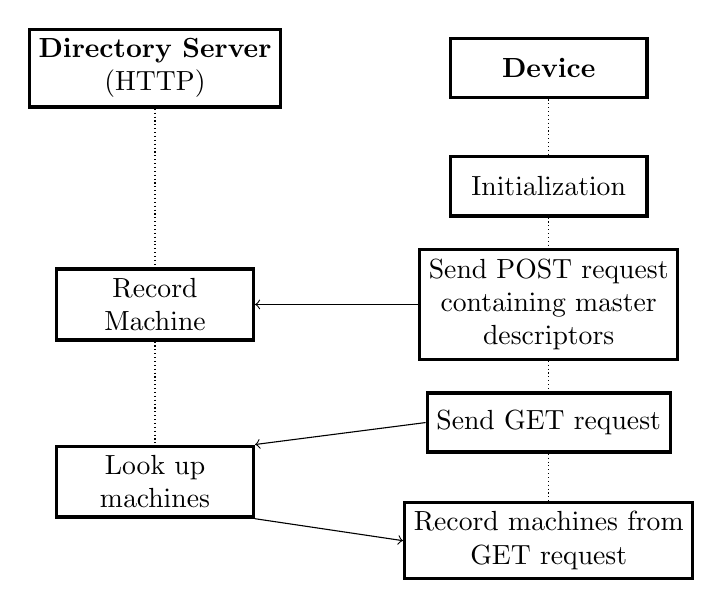
\begin{tikzpicture}[
box/.style={rectangle, draw=black, fill=white, very thick, minimum width=25mm, minimum height=7.5mm, align=center},
empty/.style=
]
\node[box](dir){\textbf{Directory Server}\\(HTTP)};
\node[box](dev)[right of = dir, node distance=5cm]{\textbf{Device}};
\node[box](init_dev)[below of = dev, node distance=1.5cm]{Initialization};
\node[box](dev_register)[below of = init_dev, node distance=1.5cm]{Send POST request\\containing master\\descriptors};
\node[box](dir_register)[left of = dev_register, node distance=5cm]{Record\\Machine};
\node[box](dev_query_get)[below of = dev_register, node distance=1.5cm]{Send GET request};
\node[empty](dir_get_guide)[left of = dev_query_get, node distance=5cm]{};
\node[box](dir_query_get)[below of = dir_get_guide, node distance=7.5mm]{Look up\\machines};
\node[box](dev_query_receive)[below of = dev_query_get, node distance=1.5cm]{Record machines from\\GET request};

\draw[densely dotted] (dir) -- (dir_register);
\draw[densely dotted] (dev) -- (init_dev);
\draw[densely dotted] (init_dev) -- (dev_register);
\draw[densely dotted] (dir_register) -- (dir_query_get);
\draw[densely dotted] (dev_register) -- (dev_query_get);
\draw[densely dotted] (dev_query_get) -- (dev_query_receive);

\draw[->] (dev_register) -- (dir_register);
\draw[->] (dev_query_get.west) -- (dir_query_get.north east);
\draw[->] (dir_query_get.south east) -- (dev_query_receive.west);

\end{tikzpicture}
\end{center}

The POST request is a machine descriptor, containing the IP addresss and public key of the target machine in the form \texttt{IP\_ADDR:HEX\_PUBLIC\_KEY}. Only a single machine may be registered at once, but several POSTs may be made to register several machines. If a given machine is re-registered with a new IP address, the old IP address is deleted and the new IP is added instead. Because devices may turn on or off, or lose internet connection, the IP address in the directory may not be the most up to date, and may not work at all. All directory server operations happen on port 80 (the standard HTTP port), and against the root (http://address/) file. Because the directory server gives publicly available information, it is not encrypted with HTTPS.

When a get request is made to the HTTP server, it will collate all known machines not at the requesting device's IP address, and send them to the device. It does this by first sending a count of how many descriptors will be sent, followed by a newline, then the descriptors alos seperated by newlines;

\texttt{4 \newline
IP\_ADDR:HEX\_PUBLIC\_KEY \newline
IP\_ADDR:HEX\_PUBLIC\_KEY \newline
IP\_ADDR:HEX\_PUBLIC\_KEY \newline
IP\_ADDR:HEX\_PUBLIC\_KEY
}

Steps 5 and 8 involve sending, and 6 and 9 involve receiving messages. Because these messages are encrypted, they have two packets; outer (unencrypted) packets directing them to their destination while providing information required to decrypt them, and inner (encrpyted) packets containing the actual function to call. The structure of the outer packet is straightforward;

\begin{table}[h]
\begin{tabular}{|p{25mm}|l|l|p{45mm}|}
\hline
\textbf{Field Name}	& \textbf{Start byte}	& \textbf{End byte}		& \textbf{Description} \\ \hline
Origin Pub					& 0									& 31							& Public Key of origin machine \\ \hline
Destination Pub			& 32								& 63							& Public Key of destination machine \\ \hline
Contents Length			& 63								& 79							& True pre-encryption length of inner packet \\ \hline
Body								& 80								& N								& Encrypted data (first 16 bytes are the Initialization Vector) \\ \hline
\end{tabular}
\end{table}

The first three (Origin and Destination Pub, Contents Length) fields are contained within the \texttt{packet\_header} struct for ease of handling. The only thing that can be told from intercepted packets, without the shared secret, is the message endpoint machines and the message length and frequency. While it may allow an attacker to deduce the general nature of the communication, they should not be able to deduce its content. SSL exposes similar information through port numbers and message lengths, and it is considered highly secure.

Once the packet has been decrypted, is parsed as an inner packet.

\begin{table}[h]
\begin{tabular}{|p{25mm}|l|l|p{45mm}|}
\hline
\textbf{Field Name}	& \textbf{Start byte}		& \textbf{End byte}		& \textbf{Description} \\ \hline
Destination I				& 0											& 11									& ID of the target machine. Used to verify packet has been decoded correctly.  \\ \hline
Function name				& 12										& 31									& Name of the function to call. Null-terminated string.  \\ \hline
On Success					& 32										& 51									& Name of the function to call on origin machine if this task completes successfully. Null-terminated string. \\ \hline
On Failure					& 52										& 71									& Name of the function to call on origin machine if this task does not complete successfully. Null-terminated string. \\ \hline
Parameter Null			& 72										& 72									& Is the parameter null? \\ \hline
Parameter						& 73										& N										& Null-terminated parameter \\ \hline
\end{tabular}
\end{table}

Like the outer packet, Function name to Parameter Null are incorporated into a struct for ease of handling. This is called \texttt{wire\_task}, and incorporates all of the information needed to execute the task, other than the origin and destination machine. The last two, as well as device-specific data are in the \texttt{task} struct. Both \texttt{wire\_task} and \texttt{task} are usually followed directly in memory by the null-terminated parameter if any exists, but this cannot be inside of the struct because it is of varying length.



\subsubsection{Nihilo API Macros}

\textbf{\texttt{NIH\_VOID(NAME, PARAMNAME)}}\newline
Create a new Nihilo-exposed function with name \texttt{NAME}, and a \texttt{const char*} parameter called \texttt{PARAMNAME}. Replaces the normal function declaration. If it is called with no parameter, \texttt{PARAMNAME} will equal \texttt{nullptr}.

\begin{tcolorbox}[colback=white,grow to left by=2.5mm,grow to right by=2.5mm,left*=0mm,right*=0mm,sharp corners]
\begin{verbatim}
NIH_VOID(entry, param){
  logStr("hello, world!);
}
\end{verbatim}
\end{tcolorbox}

\textbf{\texttt{NIH\_CHARS(NAME, PARAMNAME)}}\newline
Same as \texttt{NIH\_VOID(NAME, PARAMNAME)}, but returns a \texttt{const char *}.

\begin{tcolorbox}[colback=white,grow to left by=2.5mm,grow to right by=2.5mm,left*=0mm,right*=0mm,sharp corners]
\begin{verbatim}
NIH_CHARS(entry, param){
  return "hello, world.";
}
\end{verbatim}
\end{tcolorbox}

\textbf{\texttt{WASM\_IMPORT(MODULE,NAME)}}\newline
Internal macro, assisting with exposing functions to the user.

\subsubsection{Nihilo API Functions}

\textbf{\texttt{void mallocWasm(void** target, uint32\_t size)}}\newline
Replacement for malloc(). Pointer pointed to by \texttt{target} is is set to point to a new buffer of length \texttt{size} bytes. Allocates heap inside of wasm3's memory space.

\begin{tcolorbox}[colback=white,grow to left by=2.5mm,grow to right by=2.5mm,left*=0mm,right*=0mm,sharp corners]
\begin{verbatim}
NIH_VOID(entry, param){
  char* buf;
  mallocWasm((void**)&buf, 50);
  strcpy(buf, "test");
  logStr(buf);
}
\end{verbatim}
\end{tcolorbox}

\textbf{\texttt{void writeString(const char* path, const char* value)}}\newline
Saves \texttt{value} in \texttt{path} in the current machine's JSON. Only objects and strings are currently supported to save, and only strings to directly edit, deliniated by full stops(\texttt{.}). If the write is under an object that doesn't yet exist, it will create that object.

\begin{tcolorbox}[colback=white,grow to left by=2.5mm,grow to right by=2.5mm,left*=0mm,right*=0mm,sharp corners]
\begin{verbatim}
NIH_VOID(save_value, param){
  writeString("A.B.C.Str", param);
}
\end{verbatim}
\end{tcolorbox}

\textbf{\texttt{void readString(const char* path, char** target)}}\newline
Looks up \texttt{path} in the current machine's JSON. Pointer pointed to by \texttt{target} is set to point to the value read out of JSON.

\begin{tcolorbox}[colback=white,grow to left by=2.5mm,grow to right by=2.5mm,left*=0mm,right*=0mm,sharp corners]
\begin{verbatim}
NIH_VOID(log_value, param){
  char* val;
  readString("A.B.C.Str", &val);
  if(val != nullptr)
    logStr(val);
}
\end{verbatim}
\end{tcolorbox}

\textbf{\texttt{int knownPubs(unsigned char** IdsOut, int include\_local, int include\_non\_local)}}\newline
Lists machines currently known to this device. if \texttt{include\_local} is set to 0, machines on the device will be excluded from the list. Similarly, if \texttt{include\_non\_local} is set to 0, machines not on the device will be excluded. \texttt{IdsOut} is set to point to a list of the 32-byte public keys of the requested devices, and the function returns the number of machines which have been included in \texttt{IdsOut}.

\begin{tcolorbox}[colback=white,grow to left by=2.5mm,grow to right by=2.5mm,left*=0mm,right*=0mm,sharp corners]
\begin{verbatim}
NIH_VOID(log_value, param){
  unsigned char* ids;
  int known = knownPubs(&ids, 0, 1);
  if(known > 0)
    logStr("Devices knows of non-local machines");
}
\end{verbatim}
\end{tcolorbox}

\textbf{\texttt{void logStr(const char* tolog)}}\newline
Log a string to the user, using the ESP-IDF monitoring program.

\begin{tcolorbox}[colback=white,grow to left by=2.5mm,grow to right by=2.5mm,left*=0mm,right*=0mm,sharp corners]
\begin{verbatim}
NIH_VOID(log_value, param){
  logStr("hello, world");
}
\end{verbatim}
\end{tcolorbox}

\textbf{\texttt{void queue(const unsigned char* target\_pub, const char* fname, const char* param, const char* onsuccess, const char* onfail)}}\newline
Add a new task to the back of the queue, to be executed after every other task currently on the queue. The task will be sent to \texttt{target\_pub}, either directly if it is on this device, or through an encrypted socket if it is on another. If \texttt{target\_pub} is nullptr, it will be sent to the current machine. The target device will execute \texttt{fname(param)}, and pass its result to \texttt{onsuccess} in this machine if it is a success, or \texttt{onfail if not}. \texttt{param}, \texttt{onsuccess} and \texttt{onfail} may be set to \texttt{nullptr}, but \texttt{fname} must be a valid string.

\begin{tcolorbox}[colback=white,grow to left by=2.5mm,grow to right by=2.5mm,left*=0mm,right*=0mm,sharp corners]
\begin{verbatim}
NIH_VOID(entry, param){
  queue(nullptr, "test", "hello!", "success", nullptr);
}
NIH_CHARS(test, param){
  logStr(param);
  return "response";
}
NIH_VOID(success, param){
  logStr(param);
}
\end{verbatim}
\end{tcolorbox}
This example prints;
\begin{tcolorbox}[colback=white,grow to left by=2.5mm,grow to right by=2.5mm,left*=0mm,right*=0mm,sharp corners]
\begin{verbatim}
hello!
response
\end{verbatim}
\end{tcolorbox}
\textbf{\texttt{void setReturn (const char* ret)}}\newline
Internal function, assisting with returning data to the runtime.

\textbf{\texttt{void getParam(char** param)}}\newline
Internal function, assisting with passing the parameter from the runtime to WASM code.




\section{Results}


\section{Analysis and conclusion}


\section{Reflection}

\section{Glossary}


\section{References}
\begin{thebibliography}{9}
\bibitem{32datasheet}
	\url{https://www.espressif.com/sites/default/files/documentation/esp32_datasheet_en.pdf}
\bibitem{lx6datasheet}
	\url{https://mirrobo.ru/wp-content/uploads/2016/11/Cadence_Tensillica_Xtensa_LX6_ds.pdf}
\bibitem{asm}
	\url{http://asmjs.org/spec/latest/}
\bibitem{wasm}
	\url{https://webassembly.github.io/spec/core/_download/WebAssembly.pdf}
\bibitem{rsa}
	\url{https://people.csail.mit.edu/rivest/Rsapaper.pdf}
\bibitem{ecc}
	\url{https://www.ams.org/journals/mcom/1987-48-177/S0025-5718-1987-0866109-5/S0025-5718-1987-0866109-5.pdf}
\bibitem{aes}
	\url{https://nvlpubs.nist.gov/nistpubs/FIPS/NIST.FIPS.197.pdf}
\bibitem{createap}
	\url{https://github.com/oblique/create_ap}
\bibitem{birth}
	\url{http://www.winlab.rutgers.edu/comnet2/Reading/documents/Birthday_attack.pdf}
\bibitem{pigeon}
	\url{https://www.math.ust.hk/~mabfchen/Math391I/Pigeonhole.pdf}
\bibitem{weberror}
  \url{https://owasp.org/www-community/Improper_Error_Handling}
\end{thebibliography}
\end{document}
